%05/02 - Raúl Guantes
\chapter{Sistemas dinámicos no lineales}
\section{Crecimiento logístico}
El crecimiento de las poblaciones biológicas está limitado por la disponibilidad de recursos. Para modelar este fenómeno, se introduce un nuevo parámetro $k$, que representa la capacidad de carga del entorno, es decir, la cantidad máxima de individuos que el entorno puede sostener (la cantidad de recursos disponibles para toda la población). Además, se considera:
\begin{itemize}
\item $r$: la \textbf{tasa de crecimiento} de una población (positiva)
\item $N(t)$: el número de células en el tiempo $t$
\end{itemize}
La dinámica de la población se describe mediante una ecuación diferencial que depende de $N$, $r$ y $k$:
$$\frac{dN}{dt} = f(N; r, k)$$

\subsection{Ecuación de crecimiento logístico}
Si los recursos son ilimitados, la población crece exponencialmente:
$$\frac{dN}{dt} = rN$$

Sin embargo, cuando los recursos son limitados, el crecimiento se ve afectado por la disponibilidad de recursos. Si la población supera la capacidad de carga ($N > k$), la población disminuye debido a la falta de recursos. Por el contrario, si la población es pequeña ($N < k$), hay suficientes recursos para que la población crezca. Esto se modela mediante la \textbf{ecuación de crecimiento logístico}:
$$\frac{dN}{dt} = rN(1-\frac{N}{k})$$
Esta ecuación es \textbf{no lineal} debido al término $N^2$. Se puede obtener la derivada para ver si la población crece (derivada positiva) o disminuye (derivada negativa).

\subsection{Solución de la ecuación logística}
La solución analítica de la ecuación logística es:
$$N(t) = \frac{N(0) k}{N(0) + (k - N(0))e^{-rt}}$$
Cuando $t \rightarrow \infty$, la población tiende a la capacidad de carga $k$, alcanzando un \textbf{estado de equilibrio}:
$N(t) \rightarrow k$

\subsection{Puntos de equilibrio y estabilidad}
En un sistema dinámico, los \textbf{puntos de equilibrio} son aquellos en los que la derivada temporal es cero ($dN/dt = 0$). Para la ecuación logística, los puntos de equilibrio son:
$$0 = r N (1 - \frac{N}{K}) \begin{cases} 
N^1_{eq} = K \rightarrow \text{Estable} \\
N^2_{eq} = 0 \rightarrow \text{Inestable}
\end{cases}
$$

\begin{itemize}
\item $N_{eq} = k$ es un punto de equilibrio estable, ya que la población tiende a $k$ a largo plazo.
\item $N_{eq} = 0$ es un punto de equilibrio inestable, ya que cualquier pequeña perturbación hará que la población crezca hacia $k$.
\end{itemize}

\begin{figure}[h]
\centering
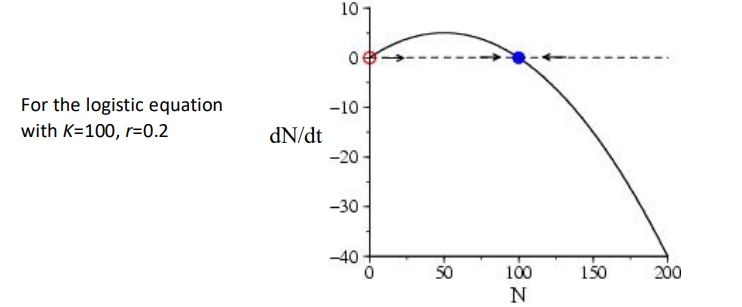
\includegraphics[width = 0.9\textwidth]{figs/estabilidad-dinamica.png}
\end{figure}

\subsection{Análisis de estabilidad}
Para entender el comportamiento a largo plazo de un sistema dinámico, es necesario calcular los puntos de equilibrio y determinar su estabilidad. 
Un sistema biológico de verdad, al medir a tiempos largos, siempre va a estar en un estado de equilibrio estable, al ser robustos a fluctuaciones. La estabilidad se puede deducir sin resolver la ecuación diferencial mediante dos formas: la forma gráfica y la forma matemática. 

\subsubsection{Método gráfico: Plano de fases}
En sistemas con una sola variable, se utiliza el plano de fases, donde:
\begin{itemize}
\item El eje x representa la variable $N$.
\item El eje y representa la derivada $dN/dt$
\end{itemize}
Para la ecuación logística:
$$\frac{dN}{dt} = f(N) = rN - \frac{rN^2}{K}$$ 
Esta función es una parábola invertida con puntos de corte en $N = 0$ y $N = k$. El máximo de la parábola se encuentra en:
$$\frac{df}{dN} = 0 \rightarrow r - \frac{2rN}{k} = 0 \rightarrow N = \frac{k}{2}$$

El punto $N = k$ es \textbf{estable} porque, a su izquierda, $dN/dt > 0$ (la población crece), y a su derecha, $dN/dt < 0$ (la población decrece).

\subsubsection{Método matemático: Linealización}
Este método es más general y puede aplicarse a sistemas con múltiples variables. Consiste en linealizar la función $f(N)$ alrededor de un punto de equilibrio $N_{eq}$ utilizando una \textbf{aproximación de Taylor}.
\begin{enumerate}
\item \textbf{Perturbación alrededor del equilibrio}
$$N = N_{eq} + \Delta N$$

\item \textbf{Derivada temporal}
$$\frac{dN}{dt} = \frac{d(N_{eq} + \Delta N}{dt} = f(N_{eq} + \Delta N)$$

\item \textbf{Aproximación de Taylor} $f(N) \approx a + bN + cN^2 + dN^3 + \ldots$
$$f(N_{eq} + \Delta N) \approx f(N_{eq}) + \frac{df(N_{eq}}{dN} \Delta N$$
Como $f(N_{eq}) = 0$ (punto de equilibrio), se simplifica a:
$$\frac{d \Delta N}{dt} \approx f'(N_{eq}) \Delta N$$

\item \textbf{Solución de la ecuación linealizada}
$$\Delta N(t) = \Delta N(0) \cdot e^{f'(N_{eq})t}$$
\begin{itemize}
\item Si $f'(N_{eq}) > 0$, el punto de equilibrio es \textbf{inestable}, ya que la perturbación crece con el tiempo.
\item Si $f'(N_{eq}) < 0$, el punto de equilibrio es \textbf{estable}, ya que la perturbación decrece con el tiempo.
\end{itemize}
\end{enumerate}